\begin{figure*}[!t]
    \centering
    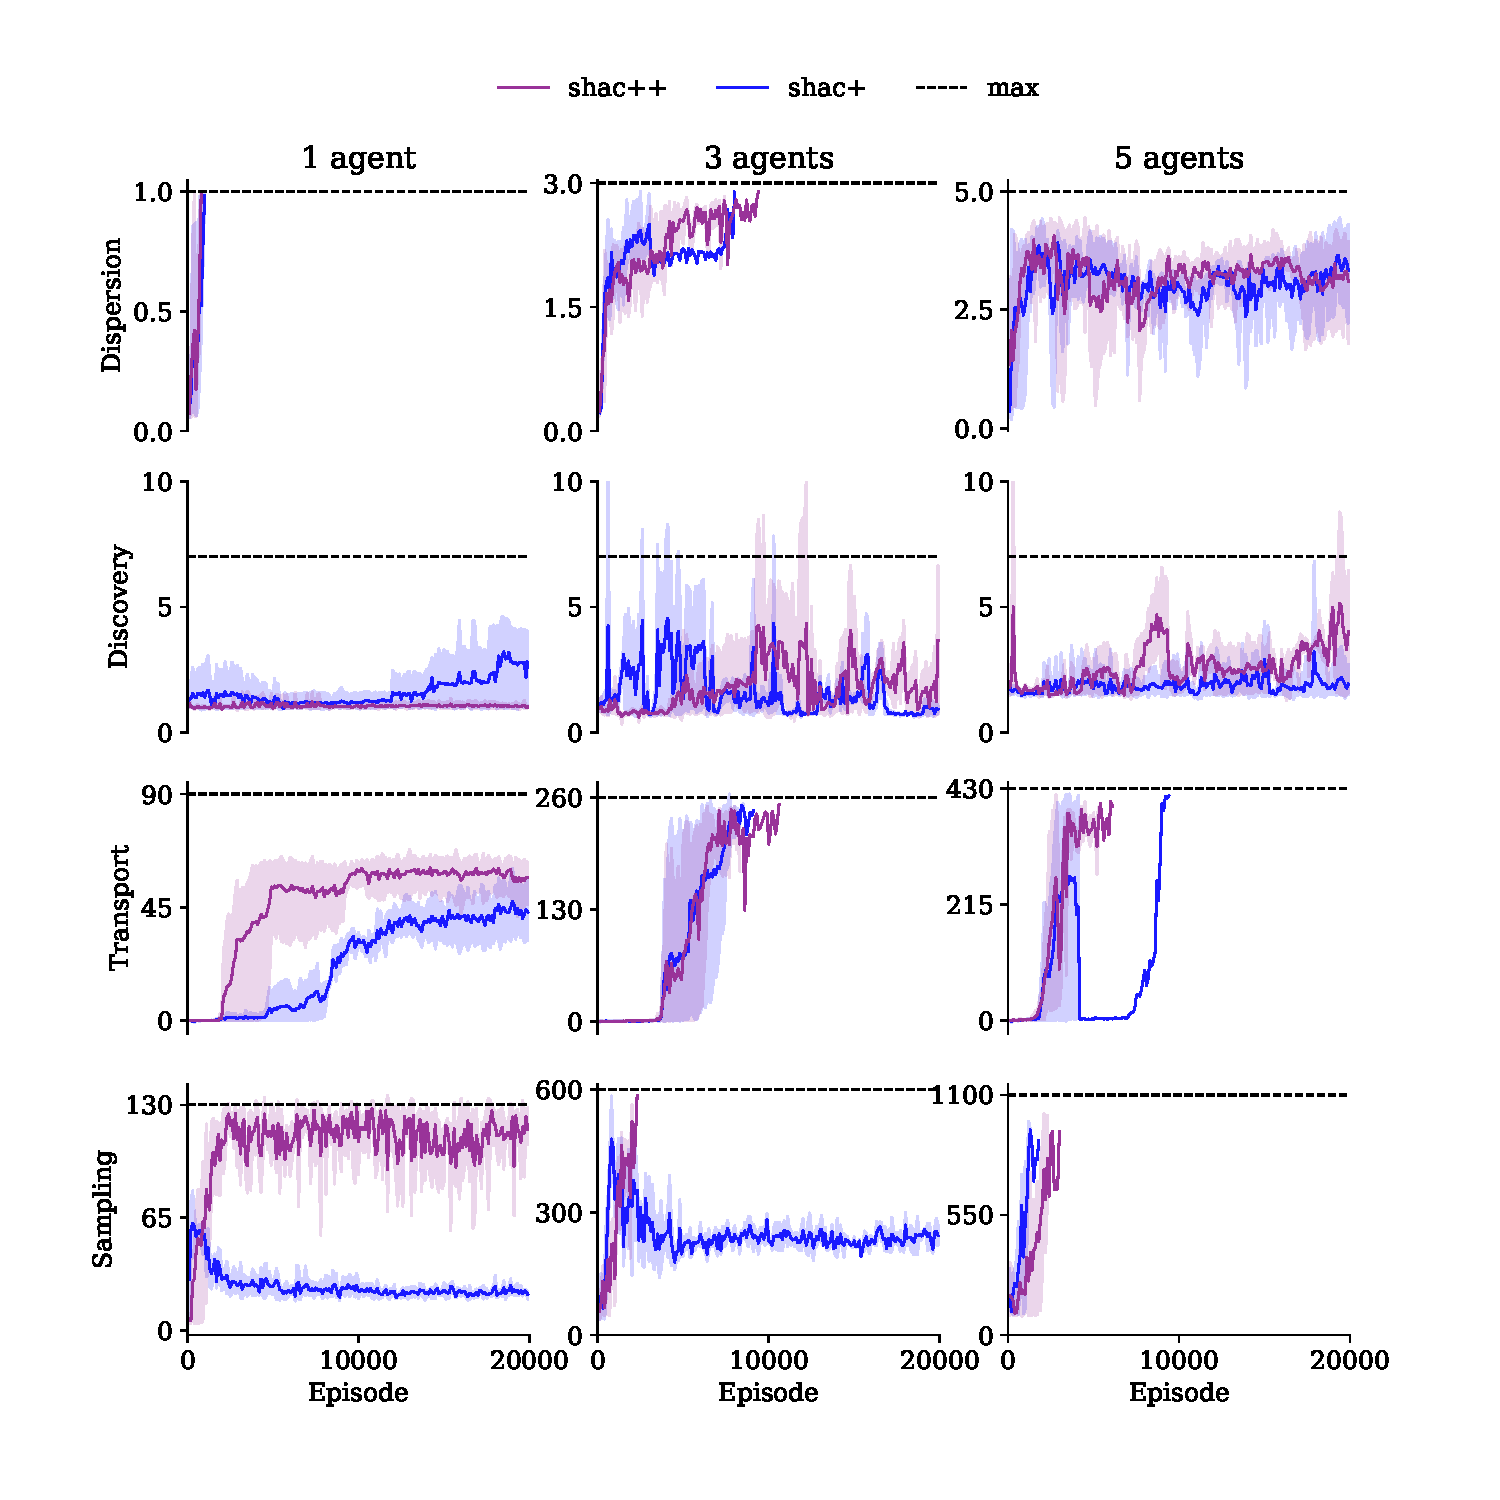
\includegraphics[width=\textwidth]{figs/ablation-transformer.pdf}
    \caption{Comparison between \fname{} with and without transition network, labelled \fnamer{}, for increasing number of agents for Dispersion, Transport, Discovery, and Sampling scenarios.}
    \label{fig:ablation}
\end{figure*}


\section{Ablation Study}\label{apx:ablation}
While we mainly focus on replacing both the reward and transition function with neural networks, we also investigate the effect of replacing only the latter. 

In fact, the transition function is the most complex component to replace as it requires modeling with precision the observations obtained from the environment after a number of $H$ actions from each agent. Avoiding the need of such network lightens the algorithm but it reintroduces the need for a differentiable environment.
\Cref{fig:ablation} presents a comparative analysis between \fname{} and \fnamer{}. The results demonstrate that utilizing the true transition function significantly impacts the performance of \fname{}. This performance difference is particularly pronounced in the Sampling and Transport scenarios, where \fname{} consistently achieves superior results compared to \fnamer{}, both in terms of maximum reward and sample efficiency. This advantage is most evident in the Sampling scenario with one and three agents.

However, the performance gap narrows in certain scenarios. For instance, in the Dispersion scenario, \fnamer{} achieves comparable performance to \fname{}. This equivalence might be attributed to the increased complexity of learning the transition function in this particular environment.
